\documentclass[utf8,xcolor=table]{beamer}

\usepackage[T2A]{fontenc}
\usepackage[utf8]{inputenc}
\usepackage[english,russian]{babel}
\usepackage{minted}
\usepackage{ulem}
\usepackage{cmap}
\usepackage{multirow}

\hypersetup{colorlinks,linkcolor=blue,urlcolor=blue}

\mode<presentation>{
	\usetheme{CambridgeUS}
}

\renewcommand{\t}[1]{\ifmmode{\mathtt{#1}}\else{\texttt{#1}}\fi}

\title{Многопоточность}
\author{Егор Суворов}
\institute[СПб АУ]{Курс <<Парадигмы и языки программирования>>, подгруппа 3}
\date[19.10.2016]{Среда, 19 октября 2016 года}

\setlength{\arrayrulewidth}{1pt}

\begin{document}

\begin{frame}
\titlepage
\end{frame}

\begin{frame}{План занятия}
	\tableofcontents
\end{frame}

\section{Параллельные вычисления}
\subsection{Зачем}

\begin{frame}
	\tableofcontents[currentsection,currentsubsection]
\end{frame}

\begin{frame}{Скорость вычислений}
	\begin{itemize}
		\item Хочется обрабатывать всё б\'{о}льшие объёмы информации всё быстрее.
		\item Пример: эмуляция движений воздуха на планете Земля за ближайшие 48 часов (прогноз погоды).
		\item Пока работает эмпирический \href{https://ru.wikipedia.org/wiki/\%D0\%97\%D0\%B0\%D0\%BA\%D0\%BE\%D0\%BD\_\%D0\%9C\%D1\%83\%D1\%80\%D0\%B0}{закон Мура}: каждые два года плотность транзисторов удваивается.
		\item Раньше это означало увеличение частоты процессора в два раза.
		\item Уже нет: процессор с частотой 2.8 ГГц был представлен в 2004 году (Pentium 4 Prescott).
		\item С тех пор скорость работы повышалась, но другими способами: размер кэша, скорость памяти, периферии...
		\item Уже уткнулись в ограничения размера процессора из-за скорости света.
	\end{itemize}
\end{frame}

\begin{frame}[fragile]{Параллелизм}
	\begin{itemize}
		\item Иногда можно работать быстрее, не увеличивая частоту, распараллелив команды:
\begin{minted}{cpp}
int x = a * b * 10;  // Нужен блок умножения.
int y = a / b;       // Нужен блок деления.
\end{minted}
		\item Процессоры умеют это автоматически детектировать без участия программистов.
		\item Компиляторы умеют передвигать операции так, чтобы процессору было проще.
		\item В последние годы активно появляются многоядерные процессоры: впихнуть второе ядро оказалось проще оптимизации физических процессов.
		\item Также можно использовать мощь б\'{о}льшего числа компьютеров (\href{https://ru.wikipedia.org/wiki/Folding@home}{Folding@Home}).
	\end{itemize}
\end{frame}

\begin{frame}{На домашнем компьютере}
	Идеи распараллеливания полезны и где-то, кроме ускорения:
	\begin{itemize}
		\item
			Обычные задачи дома не требуют большой вычислительной мощи:
			\begin{itemize}
				\item Процесс обычно ждёт реакции пользователя, диска или сети.
				\item Вычисления длятся не больше нескольких секунд.
			\end{itemize}
		\item Хочется свободно переключаться между приложениями и слушать музыку в фоне.
		\item Если есть ресурсоёмкая задача, нестрашно, если она будет выполняться чуть медленнее.
		\item На телефоне одно ядро может целиком отрисовывать нетормозящий интерфейс, а другое "--- производить вычисления.
	\end{itemize}
\end{frame}

\subsection{Как}
\begin{frame}[fragile]{Параллельные алгоритмы}
	\begin{itemize}
		\item Некоторые алгоритмы параллелятся просто:
\begin{minted}{cpp}
int sum = 0;
for (int x : values) sum += x;
\end{minted}
		\item Некоторые "--- естественно и на уровне железа:
\begin{minted}{cpp}
char buf1[100], buf2[100];
fread(file_on_disk1, 1, sizeof buf1, buf1);
fread(file_on_disk2, 1, sizeof buf2, buf2);
\end{minted}
		\item Некоторые не параллелятся:
\begin{minted}{cpp}
int steps = 0;
for (int x = 0; x != 0; x = f(x)); steps++;
\end{minted}
		\item Надо писать специальные алгоритмы для распределённых вычислений.
	\end{itemize}
\end{frame}

\begin{frame}{Иллюстрация}
	\begin{center}
		
\includegraphics[height=6cm]{cpus-joke.jpg}

		Простое добавление ядер не увеличивает производительность!
	\end{center}
\end{frame}

\begin{frame}{В прикладном хозяйстве}
	\begin{itemize}
		\item Современные ОС различают \textit{потоки} и \textit{процессы}.
		\item Процесс "--- это обычно одно приложение (браузер, IDE, веб-сервер...), у которого может быть много потоков.
		\item Например: у браузера один поток на вкладку; у веб-сервера "--- один поток на клиента.
		\item Изначально у процесса есть только один поток (\textit{главный}), он может создавать другие.
		\item Более строго: процесс "--- это некоторое множество потоков, у которых общая память и другие ресурсы (открытые файлы).
		\item Поток "--- это что-то, выполняющее некий код (есть отдельный стек, свои данные в регистрах процессора, свой код).\
	\end{itemize}
\end{frame}

\begin{frame}{С точки зрения программиста}
	\begin{itemize}
		\item На разных ОС разные методы для работы с процессами или потоками.
		\item Напрямую API уровня ОС, как обычно, никто не использует.
		\item В языке высокого уровня (Java, Python) обычно есть соответствующая библиотека.
		\item Также есть другие классические библиотеки и стандарты:
			\begin{itemize}
				\item pthread "--- Posix Thread, стандарт в C. Будем использовать.
				\item OpenMP "--- высокоуровневое распараллеливание для C/C++/Fortran.
				\item CUDA "--- вычисления на графических картах (ядер тысячи, но они умеют меньше, чем CPU).
			\end{itemize}
	\end{itemize}
\end{frame}

\begin{frame}[fragile]{Типичный псевдокод-1}
\begin{minted}{cpp}
void draw() {
    while (true) {
        wait_for_events();
        process_updates();
        process_mouse_events();
        repaint();
    }
}
int main() {
    Thread draw_thread(draw);
    draw_thread.start();
    // ...
    add_rectangle(10, 10, 30, 40);
    // ...
}
\end{minted}
\end{frame}

\begin{frame}[fragile]{Типичный псевдокод-2}
\begin{minted}{cpp}
void process_client(Client client) {
    string request = client.read();
    string answer = "I've got " + request;
    client.write(answer);
}
int main() {
    while (true) {
        Client client = get_next_client();
        Thread(process+client, client).start();
    }
}
\end{minted}
\end{frame}

\begin{frame}[fragile]{Типичный псевдокод-3}
\begin{minted}{cpp}
void merge_sort(int l, int r) {
    if (l + 1 == r) return;
    Thread t1(merge_sort, l, (l + r) / 2);
    Thread t2(merge_sort, (l + r) / 2, r);
    t1.start(); t2.start(); // Запускаем потоки.
    t1.join(); t2.join();   // Ждём завершения.
    merge(l, r);
}
\end{minted}
\end{frame}

\section{Практические грабли}
\subsection{Простое приложение на pthread}

\begin{frame}
	\tableofcontents[currentsection,currentsubsection]
\end{frame}

\begin{frame}{Что такое pthread}
	\begin{itemize}
		\item Стандартный интерфейса функций для работы с потоками (POSIX Threads).
		\item Есть реализации под Windows, Linux и другие ОС.
		\item Стандарт при разработке программ на C.
		\item Имена функций и типов начинаются с \t{pthread\_}.
		\item В Linux можно получить справку, набрав \t{man <имя функции>} в консоли.
		\item Под остальными "--- то же самое, но в гугле.
	\end{itemize}
\end{frame}

\begin{frame}[fragile]{Пример кода}
\begin{minted}{cpp}
void* worker(void* arg) {
    printf("Hello from thread! arg=%d\n", *(int*)arg);
    *(int*)arg += 10;
    return arg;
}
int main(void) {
    pthread_t id;
    int data = 1234;
    assert(pthread_create(&id, NULL, worker, &data) == 0);
    void* retval;
    assert(pthread_join(id, &retval) == 0);
    assert(retval == &data);
    printf("data is %d\n", data);
    return 0;
}
\end{minted}
\end{frame}

\begin{frame}{Как живут потоки}
	\begin{itemize}
		\item При создании потока при помощи \t{pthread\_create} указывается функция и её аргумент "--- один указатель на что угодно.
		\item Вернуть функция тоже может указатель на что угодно.
		\item Поток завершается, когда функция делает \t{return} или \t{pthread\_exit}.
		\item Указатель на поток хранится в переменной типа \t{pthread\_t}.
		\item При создании потока он сразу начинает выполняться.
		\item \t{pthread\_join} делает следующее:
			\begin{enumerate}
				\item Ждёт окончания работы потока.
				\item Освобождает все ресурсы потока (стек).
				\item Возвращает то, что вернула функция потока.
			\end{enumerate}
		\item Когда \t{main} делает \t{return 0} или вы вызываете \t{exit(0)}, умирает весь процесс со всеми потоками.
		\item Но в \t{main} можно сделать \t{pthread\_exit}, если очень хочется, тогда процесс не умрёт, пока живы потоки.
	\end{itemize}
\end{frame}

\begin{frame}[fragile]{Упражнение: сборка кода}
	\begin{enumerate}
		\item Качаем решение с \href{https://github.com/yeputons/fall-2016-paradigms/raw/master/161019/sources/01-simple.c}{GitHub}.
		\item \texttt{gcc 01-simple.c -o 01-simple -Wall -Wextra -Werror} или аналог в вашей IDE.
		\item \texttt{./01-simple}
		\item Ожидаемый вывод:
\begin{verbatim}
Hello from thread! arg=1234
data is 1244
\end{verbatim}
	\end{enumerate}
\end{frame}

\begin{frame}{Несколько замечаний про C}
	\begin{itemize}
		\item На языке C лучше включить все предупреждения компилятора (warnings), в GCC это делают ключи \t{-Wall}, \t{-Wextra}.
		\item Если вы включили предупреждения "--- их лучше сразу трактовать как ошибки (\t{-Werror}), иначе быстро научитесь их игнорировать.
		\item Если аргумент функции не используется, после него в GCC надо писать \t{\_\_attribute\_\_((unused))}.
		\item Из функции всегда надо что-то вернуть (хотя бы \t{NULL}).
		\item \href{http://codeforces.com/blog/entry/17747}{Никогда} не начинайте название переменной с нижнего подчёркивания!
		\item Константы задаются при помощи \t{\#define SOME\_CONST (value)}.
	\end{itemize}
\end{frame}

\begin{frame}[t]{Иллюстрация}
	\begin{center}
		
\includegraphics[scale=0.5]{no-werror-meme.jpg}
	\end{center}
\end{frame}

\begin{frame}[t]{Несколько замечаний про pthread}
	Про потоки и pthread:
	\begin{itemize}
		\item Использовать \t{void* arg} и возвращаемое значение для передачи данных необязательно.
		\item Вся память внутри процесса одинаково доступна всем потокам на чтение и запись.
		\item \t{void* arg} возникает только тогда, когда надо запустить потоки на разных данных.
		\item Что произойдёт, если мы забудем \t{join} и \t{main} завершится до начала \t{worker}?
			\only<2->{Неопределённое поведение "--- \t{worker} попытается изменить переменную \t{data}, которая уже исчезла.}
	\end{itemize}
\end{frame}

\begin{frame}{Кто освобождает ресурсы?}
	На самом деле в pthread есть два типа потоков: joinable и detached.

	Joinable:
	\begin{itemize}
		\item Тип по умолчанию.
		\item На таком потоке должен быть ровно один раз вызыван метод \t{pthread\_join}, который освободит ресурсы и сообщит, что поток вернул.
		\item Если не вызвать "--- ресурсы не будут освобождены до конца программы.
		\item Если вызвать дважды "--- второй вызов может уронить программу или вернуть неверный результат.
	\end{itemize}

	Detached:
	\begin{itemize}
		\item Система автоматически освободит ресурсы как только поток завершится.
		\item Нельзя вызывать \t{pthread\_join} и получать возвращаемое значение "--- его негде хранить после окончания работы.
	\end{itemize}
\end{frame}

\begin{frame}{В других системах}
	\begin{itemize}
		\item Joinable/detached также используется в Java.
		\item В Windows (не в pthread под Windows!) другая концепция:
			\begin{itemize}
				\item Указатель на поток "--- сложный объект, который надо запрашивать у ОС и освобождать (как \t{FILE*}), а не просто переменная.
				\item Ресурсы потока освобождаются, когда он завершился и на него больше нет указателей.
				\item Нет разделения joinable/detached.
				\item Если кто-то может спросить состояние потока "--- у него есть указатель, значит, ресурсы потока ещё не освобождены.
			\end{itemize}
	\end{itemize}
\end{frame}

\begin{frame}{Упражнение}
	\begin{enumerate}
		\item Измените код так, чтобы \t{data} стала глобальной переменной (после этого \t{arg} не нужен).
		\item Вызовите \t{pthread\_detach} на втором потоке после запуска.
		\item Убедитесь, что программа упала.
		\item Уберите вызов \t{pthread\_join} и \t{printf} из основного потока.
		\item Убедитесь, что второй поток не всегда успевает отработать.
		\item Добавьте вызов \t{pthread\_exit} в \t{main}.
		\item Убедитесь, что после приложение перестало закрываться до окончания работы всех потоков.
	\end{enumerate}
	\href{https://github.com/yeputons/fall-2016-paradigms/raw/master/161019/sources/02-detached.c}{Код}
\end{frame}

\subsection{Состояние гонки}

\begin{frame}
	\tableofcontents[currentsection,currentsubsection]
\end{frame}

\begin{frame}{Упражнение}
	\begin{itemize}
		\item Возьмите \href{https://github.com/yeputons/fall-2016-paradigms/raw/master/161019/sources/03-writeln-single.c}{код}.
		\item При желании можете скачать \href{https://github.com/yeputons/fall-2016-paradigms/raw/master/161019/sources/Makefile}{Makefile}.
		\item Убедитесь, что на экран выводится строка.
		\item Запустите второй поток, который выводит на экран другую строку.
		\item Найдите место, где первая строка сменяется второй.
		\item Удивитесь.
	\end{itemize}
	\href{https://github.com/yeputons/fall-2016-paradigms/raw/master/161019/sources/04-writeln-race.c}{Код}
\end{frame}

\begin{frame}{Объяснение}
	\begin{itemize}
		\item
			Потоки выполняют команды <<одновременно>>.
			Если есть доступ к общему ресурсу (экран), то порядок не определить.
		\item
			Поэтому символы выводятся вперемешку.
		\item
			\textit{Состояние гонки} (\textit{race condition}) "--- это когда результат работы зависит от того, в каком порядке потоки выполняли команды.
		\item
			Самая популярная ошибка у начинающих.
		\item
			Операция называется \textit{атомарной}, если она всегда выполняется <<за один такт>>,
			то есть другие потоки не видят её частично выполненной.
		\item
			\t{writeln} выше не атомарна.
	\end{itemize}
\end{frame}

\begin{frame}{Упражнение}
	\begin{enumerate}
		\item Сделайте счётчик:
			\begin{itemize}
				\item Второй поток в цикле увеличивает глобальную переменную \t{data} до $N = 5 \cdot 10^8$.
				\item Основной поток (\t{main}) выводит на экран текущее значение \t{data} в цикле $M = 1000$ раз.
				\item Отключите оптимизации компилятора (ключ \t{-O2} или схожий не нужен).
			\end{itemize}
		\item Убедитесь, что программа выводит на экране увеличивающиеся значения, а в конце "--- $N$.
		\item Поиграйте со значением $M$, чтобы убедиться, что в конце всегда выводится $N$.
		\item Сделайте так, чтобы основной поток выводил на экран только чётные значения \t{data} и увеличьте $M$.
		\item Что теперь происходит?
	\end{enumerate}
	Мой код:
	\href{https://github.com/yeputons/fall-2016-paradigms/raw/master/161019/sources/05-counter.c}{счётчик},
	\href{https://github.com/yeputons/fall-2016-paradigms/raw/master/161019/sources/06-even-counter.c}{чётный счётчик}.
\end{frame}

\begin{frame}{Объяснение}
	Возможная последовательность действий:
	\begin{itemize}
		\item Основной поток: \t{if (data \% 2 == 0)} $\to \t{true}$.
		\item Второй поток: \t{data++}.
		\item Основной поток: \t{printf}.
	\end{itemize}
	Как исправить?
	\pause
	\begin{itemize}
		\item Можно на каждой итерации записать значение \t{data} в локальную \t{data\_snapshot} (снимок) и работать с ним.
		\item Работает только если чтение одной переменной атомарно.
		\item Не работает, если у нас много переменных мы не можем сделать атомарный снимок (классическая задача).
	\end{itemize}
\end{frame}

\begin{frame}{Иллюстрация}
	\begin{center}
		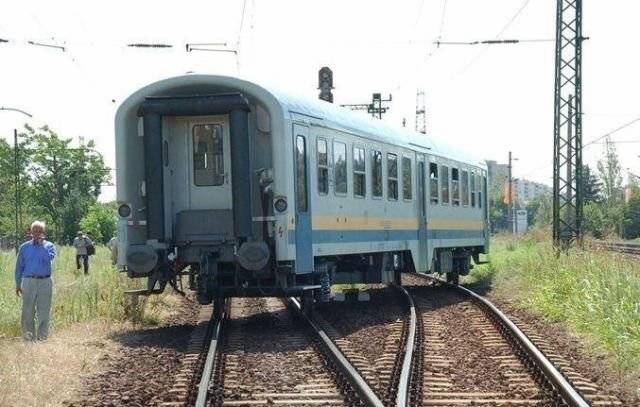
\includegraphics[scale=0.6]{race-condition.jpg}
	\end{center}
\end{frame}

\subsection{Гонка данных}
\begin{frame}{Упражнение}
	\begin{itemize}
		\item Добавьте снятие снимков в свой счётчик.
		\item Убедитесь, что все значения теперь чётные.
		\item Запустите второй поток-счётчик, который тоже увеличивает \t{data}.
		\item Что произошло?
	\end{itemize}
	Мой код:
	\href{https://github.com/yeputons/fall-2016-paradigms/raw/master/161019/sources/07-even-counter-snapshot.c}{счётчик со снимками},
	\href{https://github.com/yeputons/fall-2016-paradigms/raw/master/161019/sources/08-two-threads.c}{два счётчика}.
\end{frame}

\begin{frame}{Объяснение}
	\begin{enumerate}
		\item На уровне железа \t{data++} происходит так:
			\begin{itemize}
				\item Считай значение \t{data} из памяти.
				\item Прибавь единицу.
				\item Положи \t{data+1} на то же место в памяти.
			\end{itemize}
		\item
			Порядок операций между разными потоками произвольный.
			\begin{center}
				\begin{tabular}{cc}
					\begin{tabular}{l|c}
						Операция & \t{data} \\ \hline
						1: \t{read} $\to 10$ & 10 \\
						1: \t{+1} $\to 11$ & 10 \\
						1: \t{write(11)} & 11 \\
						2: \t{read} $\to 11$ & 11 \\
						2: \t{+1} $\to 12$ & 11 \\
						2: \t{write(12)} & 12 \\
					\end{tabular}
					&
					\begin{tabular}{l|c}
						Операция & \t{data} \\ \hline
						1: \t{read} $\to 10$ & 10 \\
						1: \t{+1} $\to 11$ & 10 \\
						2: \t{read} $\to 10$ & 10 \\
						2: \t{+1} $\to 11$ & 10 \\
						1: \t{write(11)} & 11 \\
						2: \t{write(11)} & 11 \\
					\end{tabular}
				\end{tabular}
			\end{center}
	\end{enumerate}
\end{frame}

\begin{frame}{А что вообще атомарно?}
	\begin{center}
		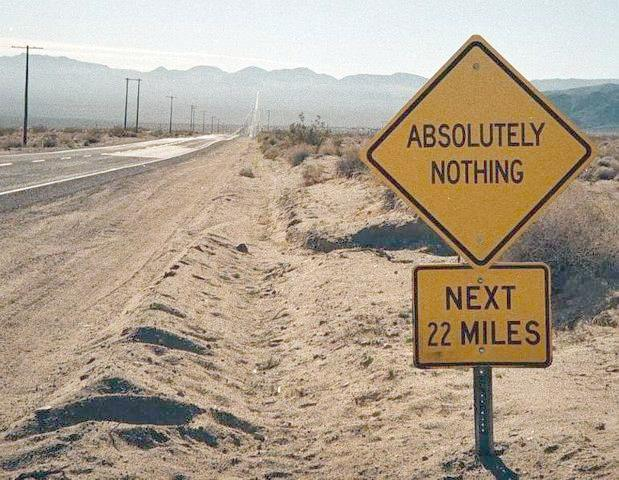
\includegraphics[scale=0.4]{absolutely-nothing.jpg}
	\end{center}
\end{frame}

\begin{frame}{Полезные советы}
	\begin{itemize}
		\item
			Что атомарно "--- очень сильно зависит от платформы, языка и ключей компиляции
			(<<модель памяти>>).
		\item Не пытайтесь угадать.
		\item Не пытайтесь самостоятельно писать код, зависящий от атомарности.
		\item В некоторых языках бывает \t{AtomicInteger} и похожие структуры.
		\item За ними тоже надо аккуратно следить, обычно не используют.
	\end{itemize}
\end{frame}

\subsection{Взаимное исключение}

\begin{frame}
	\tableofcontents[currentsection,currentsubsection]
\end{frame}

\begin{frame}{Как избежать гонок}
	\begin{itemize}
		\item Можно обозначить кусок кода как \textit{критическую секцию} (critical section).
		\item Каждую критическую секцию может выполнять максимум один поток.
		\item
			Если весь доступ к общим данным обозначить как критическую секцию,
			то он станет де-факто атомарным.
		\item С каждой критической секцией ассоцириуется \textit{блокировка} (lock).
		\item При входе в секцию блокировку надо \textit{взять}/\textit{захватить} (acquire).
		\item При выходе из секции блокировку надо \textit{отпустить} (unlock/release).
		\item Другие названия блокировок: монитор (monitor), мьютекс (mutex, \textbf{mut}al \text{ex}clusion).
		\item Обычно реализованы на уровне ОС и все операции с ними медленные.
	\end{itemize}
\end{frame}

\begin{frame}[fragile]{Некорректный пример}
\begin{minted}{cpp}
int data;
void* worker(void* arg __attribute__((unused))) {
  pthread_mutex_t m;
  pthread_mutex_init(&m, NULL);
  for (int i = 0; i < N; i++) {
    pthread_mutex_lock(&m);
    data++;
    pthread_mutex_unlock(&m);
  }
  pthread_mutex_destroy(&m);
  return NULL;
}
\end{minted}
\href{https://github.com/yeputons/fall-2016-paradigms/raw/master/161019/sources/09-two-threads-bad-mutex.c}{Код}.
\end{frame}

\begin{frame}[fragile]{Корректный пример}
\begin{minted}{cpp}
int data;
pthread_mutex_t m;
void* worker(void* arg __attribute__((unused))) {
  for (int i = 0; i < N; i++) {
    pthread_mutex_lock(&m);
    data++;
    pthread_mutex_unlock(&m);
  }
  return NULL;
}
// ...
  pthread_mutex_init(&m, NULL);
// ...
  pthread_mutex_destroy(&m);
// ...
\end{minted}
\end{frame}

\begin{frame}{Упражнение}
	\begin{enumerate}
		\item Добавьте mutex в \href{https://github.com/yeputons/fall-2016-paradigms/raw/master/161019/sources/08-two-threads.c}{двойной счётчик}.
		\item Уменьшите $N$ на несколько порядков (mutex'ы сильно замедляют программу).
		\item Убедитесь, что всегда выводится $2N$.
		\item Добавьте mutex в \href{https://github.com/yeputons/fall-2016-paradigms/raw/master/161019/sources/04-writeln-race.c}{writeln}.
	\end{enumerate}
	\href{https://github.com/yeputons/fall-2016-paradigms/raw/master/161019/sources/10-two-threads-good-mutex.c}{Исправленный двойной счётчик},
	\href{https://github.com/yeputons/fall-2016-paradigms/raw/master/161019/sources/11-writeln-mutex.c}{исправленный writeln}.
\end{frame}

\begin{frame}[fragile]{Блокировка}
	\begin{itemize}
		\item \t{pthread\_mutex\_lock} блокируется и ждёт, пока блокировка не станет доступна для захвата.
		\item Есть ли проблемы в следующем псевдокоде?
\begin{minted}{cpp}
void thread1() {
  m1.lock(); m2.lock();
  // ...
  m2.unlock(); m1.unlock();
}
void thread2() {
  m2.lock(); m1.lock();
  // ...
  m1.unlock(); m2.unlock();
}
\end{minted}
	\end{itemize}
\end{frame}

\begin{frame}{Взаимная блокировка}
	\begin{center}
		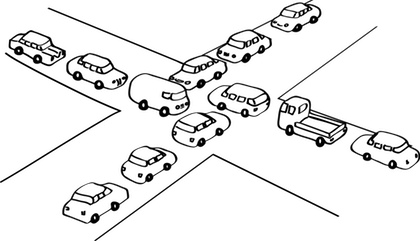
\includegraphics{deadlock.jpg}
	\end{center}
	\begin{itemize}
		\item
			Может случиться проблема:
			\begin{enumerate}
				\item Поток 1 захватывает \t{m1}.
				\item Поток 2 захватывает \t{m2}.
				\item Поток 1 не может захватить \t{m2}.
				\item Поток 2 не может захватить \t{m1}.
				\item Оба потока встали в \textit{deadlock} (\textit{взаимная блокировка}).
			\end{enumerate}
		\item
			Решение: всегда брать блокировки в одном и том же порядке.
			Тогда можно доказать, что deadlock такого вида не образуется.
		\item
			Если ввести линейный порядок на mutex не получается, у вас проблема.
	\end{itemize}
\end{frame}

\begin{frame}[fragile]{Reentrant}
\begin{minted}{cpp}
void inc() {
  m.lock(); data++; m.unlock();
}
void double_inc() {
  m.lock(); inc(); inc(); m.unlock();
}
\end{minted}
	\begin{itemize}
		\item \t{double\_inc} заблокируется, так как \t{inc} попробует взять mutex второй раз.
		\item Есть специальный вид mutex, которые позволяют захватывать себя ещё раз из того же потока, называется \textit{reentrant}.
		\item Их обычно не используют "--- они сложнее в реализации.
		\item
			Решение: ввести <<приватную>> функцию \t{inc\_lock\_held}, которая предполагает,
			что mutex уже взят.
	\end{itemize}
\end{frame}

\begin{frame}{Резюме}
	\begin{itemize}
		\item Атомарные операции в потоках могут выполняться в любом порядке, если их не синхронизировать.
		\item Вы обычно не знаете, что атомарно, а что нет.
		\item \textit{Любой} доступ к общим ресурсам должен быть \textit{защищён} (guarded) блокировкой.
		\item Блокировки надо брать всегда в одном и том же порядке.
		\item TODO
	\end{itemize}
\end{frame}

\begin{frame}{Иллюстрация}
	
\end{frame}

\subsection{Не пытайтесь повторить это дома}

\begin{frame}
	\tableofcontents[currentsection,currentsubsection]
\end{frame}

\begin{frame}[fragile]{Загадка}
	Что произойдёт при запуске \href{https://github.com/yeputons/fall-2016-paradigms/raw/master/161019/sources/12-optimizer.c}{кода}?
	Предполагаем, что запись и чтение \t{int} атомарны.
\begin{minted}{cpp}
int data;
void* worker(void* arg __attribute__((unused))) {
    for (;;) {
        data++;
    }
}
// ...
    while (data < 100);
    printf("Done\n");
// ...
\end{minted}
	\begin{itemize}
		\pause\item Race condition отсутствуют.
		\pause\item Он зависнет.
		\pause\item И никогда не выведет \t{Done}.
	\end{itemize}
\end{frame}

\begin{frame}{Разгадка}
	\begin{center}
		
\includegraphics[scale=0.3]{optimizer.jpg}
	\end{center}
	Как обычно в C/C++.
\end{frame}

\begin{frame}{Подробная разгадка}
	\begin{itemize}
		\item Компилятор по умолчанию ничего про потоки не знает.
		\item Очевидно, что \t{while (data < 100);} переменную \t{data} изменить не может.
		\item Соответственно, переменная \t{data} никак измениться не может.
		\item Значит, \t{data < 100} всегда истинно, можно заменить на \t{true}.
		\item Получаем бесконечный цикл.
			\begin{center}
				
\includegraphics[scale=0.3]{win-lose.jpg}
			\end{center}
	\end{itemize}
\end{frame}

\begin{frame}[fragile]{volatile}
	Изменим \href{https://github.com/yeputons/fall-2016-paradigms/raw/master/161019/sources/13-volatile.c}{код}:
\begin{minted}{cpp}
volatile int data;  // Обозначили переменную volatile.
void* worker(void* arg __attribute__((unused))) {
    for (;;) {
        data++;
    }
}
// ...
    while (data < 100);
    printf("Done\n");
// ...
\end{minted}
	\begin{itemize}
		\item \t{volatile} говорит компилятору честно сохранять/читать значение этой переменной из памяти каждый раз, когда написано.
		\item Есть ли проблемы? \pause Пока нет.
	\end{itemize}
\end{frame}

\begin{frame}[fragile]{Reordering}
	Эквивалентны ли два куска кода?
	\begin{tabular}{p{0.4\textwidth}p{0.4\textwidth}}
		\centering
\begin{minted}{cpp}
int data, finished;
// ...
data = 123;
finished = 1;
\end{minted}
&
\begin{minted}{cpp}
int data, finished;
// ...
finished = 1;
data = 123;
\end{minted}
	\end{tabular}
	\pause
	\begin{itemize}
		\item Эквивалентны. Оптимизатор тоже так считает.
		\pause\item И может переставить местами: всё равно никто не заметит.
		\pause\item А что, если в другом потоке было так?
\begin{minted}{cpp}
if (finished) {
    printf("%d\n", data);
}
\end{minted}
	\end{itemize}
\end{frame}

\begin{frame}{Иллюстрация}
	\begin{center}
		
\includegraphics[scale=0.2]{race-condition-knock-knock.jpg}
	\end{center}
\end{frame}

\begin{frame}{Reordeing возвращается}
	\begin{itemize}
		\item Даже если одна переменная помечена как \t{volatile}, компилятор может изменить порядок записи/чтения.
		\item А вот если обе "--- не может. Проблема решена? \pause
		\item В процессоре тоже есть оптимизатор.
		\item Он тоже может переставлять инструкции как захочет, а \t{volatile} действует только на компилятор.
		\item Есть специальные ассемблерные инструкции (<<барьеры памяти>>), которые действуют на процессор.
		\item Не надо сразу пытаться в этом разобраться.
		\item \t{volatile} не предназначен для многопоточности, он нужен для других целей (memory-mapped I/O).
		\item В любом случае, иногда один поток может встретить состояние, которое было бы невозможно получить, исполняя инструкции последовательно.
	\end{itemize}
\end{frame}

\begin{frame}{А что же mutex?}
	\begin{itemize}
		\item В разных языках/библиотеках разные модели памяти (потом должны подробно рассказать про Java).
		\item Обычно везде считается, что в следующих случаях происходит (почти) полная синхронизация памяти между двумя потоками:
			\begin{enumerate}
				\item $A$ взял мьютекс, который $B$ недавно отпустил (возможно, его брал ещё кто-то).
				\item $A$ создал поток $B$.
				\item $A$ подождал завершения потока $B$.
			\end{enumerate}
		\item Все нужные барьеры памяти и прочее уже вшиты внутрь мьютексов и работы с потоками.
	\end{itemize}
\end{frame}

\begin{frame}[fragile]{Пример}
\begin{minted}{cpp}
// Thread 1
started = true;
m.lock(); data++; m.unlock();
finished1 = true;
finished2 = true;
// Thread 2
m.lock(); m.unlock();
if (finished2) {
    assert(started);    // Верно
    assert(data > 0);   // Верно
    assert(finished1);  // Может быть неверно
}
\end{minted}
	Если убрать из второго потока мьютекс "--- ничего не знаем.
\end{frame}

\begin{frame}[fragile]{Резюме}
	\begin{itemize}
		\item Если вы что-то не защитили мьютексом, можно огрести из-за reordering, даже если всё <<очевидно должно работать>>.
		\item Если всё защищено мьютексом и вы ничего не предполагаете о происходящем за пределами критических секций "--- не о чем беспокоиться.
		\item Ничего сложнее <<взяли один глобальный мьютекс перед операцией, отпустили в конце>> обычно не требуется (в том числе в дз).
		\item Любой сколько-нибудь более сложный контроль требует понимания модели памяти.
		\item
			Все проблемы "--- от общих ресурсов (переменные, файлы, экран).
			Поэтому стараются минимизировать их количество.
		\item Нет общих ресурсов "--- нет проблем.
	\end{itemize}
\end{frame}

\section{Обмен сообщениями}
\subsection{Простая реализация}

\begin{frame}
	\tableofcontents[currentsection,currentsubsection]
\end{frame}

\begin{frame}{Зачем}
	Довольно часто потоки не совсем независимы, а хотят взаимодействовать между собой.

	Классическая задача:
	\begin{itemize}
		\item Есть очередь задач.
		\item Один поток генерирует данные (producer) и добавляет их в очередь.
		\item Второй поток должен брать добавленные данные по очереди (consumer) и что-то с ними делать.
	\end{itemize}
	Например:
	\begin{itemize}
		\item Первый поток ждёт ввода с клавиатуры и кладёт считанные данные в буфер.
		\item Второй поток выполняет введённые команды (которые могут занять долгое время).
		\item Мы хотим уметь вводить команды, даже если предыдущая ещё выполняется.
	\end{itemize}
\end{frame}

\begin{frame}[fragile]{Потокобезопасная очередь}
\begin{minted}{cpp}
class ThreadsafeQueue {
    ThreadsafeQueue() { pthread_mutex_init(&m, NULL); }
    ~ThreadsafeQueue() { pthread_mutex_destroy(&m); }
    void push(int x) {
        pthread_mutex_lock(&m);
        q.push(x);
        pthread_mutex_unlock(&m);
    }
    int pop() { ... }
    bool empty() { ... }
private:
    pthread_mutex_t m;
    queue<int> q;
};
\end{minted}
\end{frame}

\begin{frame}[fragile]{Первая попытка}
	Producer:
\begin{minted}{cpp}
while (true) {
    int data = get_data();
    q.push(data);
}
\end{minted}
	Consumer:
	\pause
\begin{minted}{cpp}
while (true) {
    while (q.empty()) {
    }
    process_data(q.pop());
}
\end{minted}
\end{frame}

\begin{frame}{Проблемы}
	\begin{itemize}
		\item Если несколько COnsumer'ов, то есть race condition.
		\item Consumer активно ждёт событие от первого и тратит процессорное время.
		\item Даже если ничего не происходит, программа потребляет 100\% CPU.
		\item Consumer постоянно берёт и отпускает mutex, мешая producer'у.
		\pause
		\item
			А если добавить задержку в consumer (проверять только каждые $X$ мс),
			то сильно увеличится задержка в обработке.
		\item Без новых \textit{примитивов синхронизации} не обойтись.
	\end{itemize}
\end{frame}

\subsection{События}

\begin{frame}[fragile]{Новый примитив}
	Введём примитив \t{Event} с двумя методами:
	\begin{itemize}
		\item \t{e.wait()} "--- усыпляет поток.
		\item \t{e.notify()} "--- будит уснувший поток.
	\end{itemize}
	\begin{tabular}{p{0.45\linewidth}p{0.45\linewidth}}
		\centering
\begin{minted}{cpp}
// Producer
while (true) {
  int data = get_data();
  q.push(data);
  e.notify();
}
\end{minted}
&
\begin{minted}{cpp}
// Consumer
while (true) {
  if (!q.empty()) {
    process_data(q.pop());
  } else {
    e.wait();
  }
}
\end{minted}
	\end{tabular}
	Есть ли проблемы в коде выше?
	\pause
	Проблемы есть.
\end{frame}

\begin{frame}{Ну вы поняли}
	\begin{center}
		
\includegraphics[scale=0.4]{race-condition-everywhere.jpg}
	\end{center}
\end{frame}

\begin{frame}{Чуть подробнее}
	\begin{enumerate}
		\item Consumer проверяет \t{!global\_queue.empty()}
		\item Producer добавляет данные.
		\item Producer вызывает \t{e.notify()}, а будить некого.
		\item Consumer вызывает \t{e.wait()} и засыпает навечно.
	\end{enumerate}
	Что делать?
\end{frame}

\begin{frame}{Первый подход}
	\begin{itemize}
		\item Можно сказать, что если в момент вызова \t{e.notify()} никто не спит, то будет разбужен следующий попытающийся уснуть.
		\item Другими словами, у \t{Event} теперь есть состояние: просигналили или нет.
		\item \t{e.notify()} "--- устанавливает флаг <<просигналили>> и будит все потоки.
		\item \t{e.wait()} "--- ждёт, пока флаг установят (или не ждёт, если уже установлен) и сбрасывает его.
		\item Решает задачу producer-consumer.
		\item Используются в Windows API.
	\end{itemize}
	Однако:
	\begin{itemize}
		\item Дополнительное состояние вносит сложность "--- за ним надо следить и добавлять инвариант.
		\item В pthread не входят и под Linux обычно не используются.
	\end{itemize}
\end{frame}

\begin{frame}[fragile]{Второй подход: добавим мьютексов?}
	\begin{tabular}{p{0.45\linewidth}p{0.45\linewidth}}
		\centering
\begin{minted}{cpp}
// Producer
while (true) {
  int data = get_data();
  pthread_mutex_lock(&m);
  q.push(data);
  e.notify();
  pthread_mutex_unlock(&m);
}
\end{minted}
&
\begin{minted}{cpp}
// Consumer
while (true) {
  pthread_mutex_lock(&m);
  if (!q.empty()) {
    process_data(q.pop());
  } else {
    e.wait();
  }
  pthread_mutex_unlock(&m);
}
\end{minted}
	\end{tabular}
	Теперь race condition отсутствует.
	\pause
	Зато есть deadlock: producer не может ничего писать, пока consumer спит.
\end{frame}

\subsection{Условные переменные}

\begin{frame}{Условные переменные}
	\begin{itemize}
		\item Нам нужна атомарная операция <<отпусти мьютекс и жди события>>.
		\item Такой примитив синхронизации в pthread (и вообще много где) называется \textit{условная переменная} (conditional variable).
		\item Смысл: условная переменная "--- это способ оповещать потоки о \textit{возможном} изменении некоторого \textit{условия}, защищённого мьютексом.
		\item Ожидание пассивное, ресурсы CPU не тратятся.
		\item На каждое условие создаётся условная переменная.
		\item Поток, изменивший условие, может разбудить либо все ожидающие потоки (\t{signal}), либо один случайный (\t{broadcast}).
		\item Бывают spurious wakeup "--- система иногда может разбудить ждущий поток, даже если никто не вызывал \t{signal}/\t{broadcast}.
		\item Поэтому важно проверять условие после пробуждения.
	\end{itemize}
\end{frame}

\begin{frame}[fragile]{Создание}
	Точно так же, как и мьютекс:
\begin{minted}{cpp}
pthread_cond_t cond;
pthread_cond_init(&cond);
// ...
pthread_cond_destroy(&cond);
\end{minted}
\end{frame}

\begin{frame}[fragile]{Оповещение}
\begin{minted}{cpp}
pthread_mutex_t m;
pthread_cond_t cond; // GUARDED_BY(m)
bool some_condition; // GUARDED_BY(m)
// ...
pthread_mutex_lock(&m);
// Следующие две строки в любом порядке.
some_condition = true;
pthread_cond_signal(&cond);
pthread_mutex_unlock(&m);
\end{minted}
\end{frame}

\begin{frame}[fragile]{Ожидание условия}
\begin{minted}{cpp}
pthread_mutex_t m;
pthread_cond_t cond; // GUARDED_BY(m)
bool some_condition; // GUARDED_BY(m)
// ...
pthread_mutex_lock(&m);
while (!some_condition) {
  // Атомарно снимает мьютекс и начинает ожидание
  pthread_cond_wait(&cond, &m);
  // После выхода из cond_wait мьютекс снова захвачен.
}
pthread_mutex_unlock(&m);
\end{minted}
\end{frame}

\begin{frame}{Упражнение}
	\begin{enumerate}
		\item Возьмите реализацию с producer-consumer с \href{https://github.com/yeputons/fall-2016-paradigms/raw/master/161019/sources/14-prod-cons.c}{GitHub}.
		\item Запустите и убедитесь, что на каждую введённую строчу отзывается второй поток: сначала сразу, а потом через две секунды.
		\item Убедитесь, что если во время ожидания второго потока ввести новую строчку, то на неё второй поток тоже среагирует.
		\item Убедитесь, что если во время ожидания ввести две новых строчки, то будет обработана только последняя.
		\item Задайте все вопросы по коду; поймите, зачем нужна и что делает каждая строчка.
		\item Есть ли проблемы в этом коде?
	\end{enumerate}
\end{frame}

\begin{frame}{Конечно, есть!}
	\begin{center}
		
\includegraphics[scale=0.4]{multithreading-aliens.jpg}
	\end{center}
\end{frame}

\begin{frame}[t,fragile]{Проблема}
	Вот тут возникает race condition:
\begin{minted}{cpp}
while (true) {
    fgets(str, sizeof str, stdin);
    pthread_mutex_lock(&m);
    str_available = true;
    pthread_cond_signal(&cond);
    pthread_mutex_unlock(&m);
}
\end{minted}
	\pause
	\begin{itemize}
		\item \t{fgets} меняет буфер, который также читается из другого потока.
		\item Значит, буфер должен быть защищён мьютексом на всех стадиях.
		\item Если поменяем \t{fgets} и \t{pthraed\_mutex\_lock} местами, то\only<1>{...}\only<2->{ будет deadlock: consumer не может читать данные, пока producer ждёт.}
		\only<3->{
		\item
			Правильно сначала считать в локальную переменную, а потом скопировать в буфер.
			\href{https://github.com/yeputons/fall-2016-paradigms/raw/master/161019/sources/15-prod-cons-fixed.c}{Код}.
		}
	\end{itemize}
\end{frame}

\begin{frame}{Резюме}
	\begin{itemize}
		\item Условные переменные нужны там и только там, где поток ждёт некоторое условие.
		\item А это условие всегда защищено ровно одним мьютексом (почему?)
		\item Соответственно, условная переменная тоже защищена ровно одним мьютексом.
		\item Условие всегда надо проверять в цикле.
		\item
			\t{pthread\_cond\_wait} "--- это лишь оптимизация.
			Если её убрать, программа должна остаться корректной.
		\item
			Никакого внутреннего состояния у условной переменной нет,
			из-за этого она просто реализуется в ОС, но программисту
			надо самому явно формулировать условие, которого ждёт поток.
	\end{itemize}
\end{frame}

\begin{frame}{Необязательное упражнение на дом}
	Реализуйте Windows Event через conditional variable:
	\begin{itemize}
		\item Объект <<событие>> с методами \t{wait} и \t{notify}.
		\item В каждый момент не более одного потока ждёт (\t{wait}).
		\item Метод \t{notify} либо пробуждает ждущий поток, либо делает так, что следующий метод \t{wait} мгновенно завершится.
	\end{itemize}
	Можно создать отдельную папку в репозитории и прислать код на проверку (в теме "--- \t{[add-161019]}).

	Сигнатура:
	\begin{itemize}
		\item \t{typedef ... event\_t;}
		\item \t{event\_init(event\_t*)}
		\item \t{event\_wait(event\_t*)}
		\item \t{event\_notify(event\_t*)}
		\item \t{event\_destroy(event\_t*)}
	\end{itemize}
\end{frame}

\section{Бонус}

\begin{frame}
	\tableofcontents[currentsection,currentsubsection]
\end{frame}

\begin{frame}{Стандартные паттерны-1}
	\begin{itemize}
		\item
			\textbf{Пул потоков} (thread pool):
			\begin{itemize}
				\item Создание потоков на короткие задачи "--- это очень неэффективно.
				\item Поддерживается пул из некоторого числа потоков (примерно по числу ядер).
				\item Задачу можно отправить в пул, она выполнится в одном из потоков, когда тот освободится.
				\item Ограничивает число одновременно выполняющихся задач.
			\end{itemize}
		\item
			\textbf{Блокировка чтения-записи} (readers-writer lock)
			\begin{itemize}
				\item Как мьютекс, но позволяет потоку указать режим доступа: <<чтение>> или <<запись>>.
				\item Читателей может быть сколько угодно.
				\item Если кто-то пишет, то другие потоки ждут.
				\item Ускоряет доступ к редко меняющимся данным.
			\end{itemize}
	\end{itemize}
\end{frame}

\begin{frame}{Стандартные паттерны-2}
	\begin{itemize}
		\item
			\textbf{Акторы} (actors)
			\begin{itemize}
				\item Небольшие потоки, не имеющие общих ресурсов.
				\item Для обмена информацией посылают друг другу неизменяемые \textit{сообщения}.
				\item Вся синхронизация сконцентрирована в системе обмена сообщениями.
			\end{itemize}
		\item
			\textbf{Неблокирующие} (lock-free) структуры данных
			\begin{itemize}
				\item Работают поверх атомарных операций и моделей памяти.
				\item Не требуют блокировок или мьютексов.
				\item Работают быстрее, так как многие операции атомарны в железе и не требуют вмешательства ОС.
			\end{itemize}
	\end{itemize}
\end{frame}

\begin{frame}{Как отлаживать}
	\begin{center}
		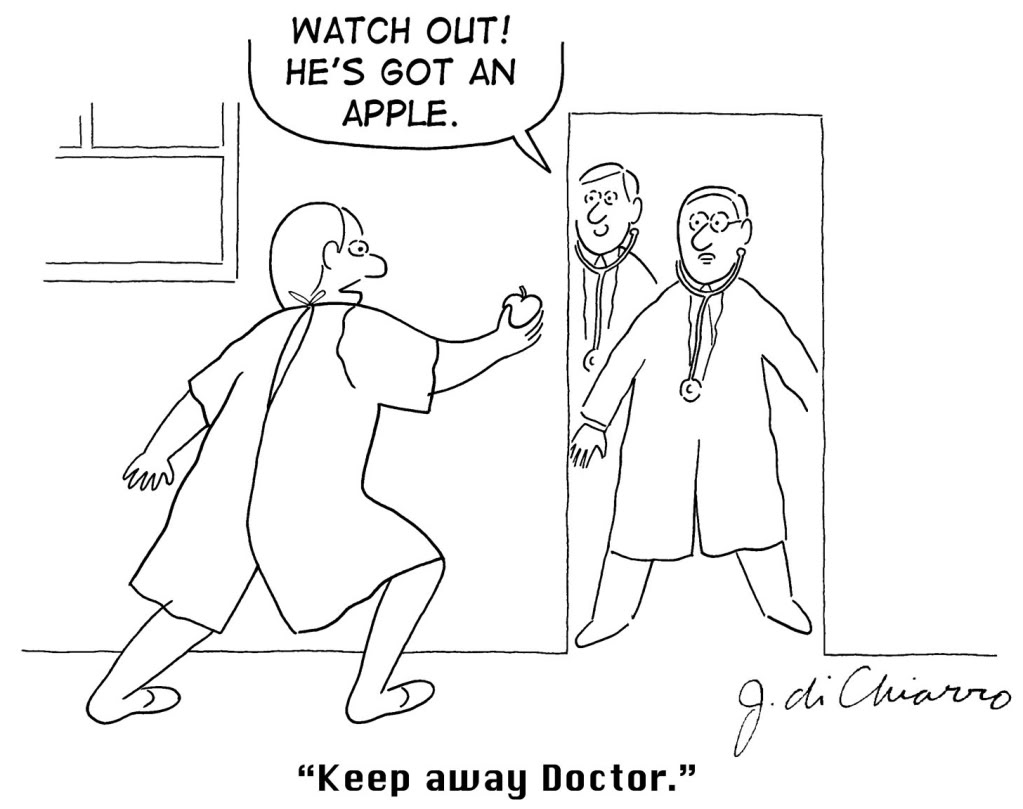
\includegraphics[scale=0.2]{apple-a-day.jpg}
		\pause

		An apple a day keeps the doctor away.

		Лучше предотвращать, чем отлаживать.
	\end{center}
\end{frame}

\begin{frame}{Причина}
	\begin{center}
		
\includegraphics[scale=0.2]{race-or-bug.jpg}
	\end{center}
	\begin{itemize}
		\item Многопоточные баги обычно тесно связаны с порядком выполнения операций.
		\item Операции выполняются в разном порядке каждый запуск, под отладчиком, в разном коде.
		\item Очень сложно ловить баг <<за руку>>.
		\item Корректная работа на куче тестов не означает отсутствие багов.
	\end{itemize}
\end{frame}

\begin{frame}{Как предотвращать}
	\begin{itemize}
		\item Явно расставляйте инварианты в комментариях: что чем защищено, в каком порядке захватывать мьютексы.
		\item Нарисуйте на бумажке все возможные состояния системы и проверьте, что инварианты выполняются.
		\item Минимизируйте количество мьютексов, если нет проблем со скоростью работы.
		\item Не используйте для синхронизации ничего, кроме мьютексов (в частности, явных \t{sleep} в программе быть не должно).
	\end{itemize}
\end{frame}

\begin{frame}{Как тестировать}
	\begin{itemize}
		\item Запускайте на больших тестах, в которых потоки работают медленно и часто происходит переключение.
		\item
			Если вы под 64-битным Linux "--- используйте thread sanitizer (добавьте ключи \t{-g -fsanitize=thread -O2 -fPIC -pie}).
			Он хорош в нахождении некоторых гонок данных, \textit{происходящих во время выполнения}.
		\item
			Для аналогичных целей можно использовать Valgrind.
		\item
			На Windows можно поставить виртуальную машину.
	\end{itemize}
\end{frame}

\begin{frame}[fragile]{Пример вывода Thread Sanitizer-1}
	На \href{https://github.com/yeputons/fall-2016-paradigms/raw/master/161019/sources/08-two-threads.c}{примере с двумя счётчиками} находит гонку сразу,
	во время первых выводов на экран:
\begin{verbatim}
==================
WARNING: ThreadSanitizer: data race (pid=13170)
  Read of size 4 at 0x7f31e00e12cc by thread T2:
    #0 worker .../08-two-threads.c:10 (...)
    #1 <null> <null>:0 (libtsan.so.0+0x000000032d69)

  Previous write of size 4 at 0x7f31e00e12cc by thread T1:
    #0 worker .../08-two-threads.c:12 (...)
    #1 <null> <null>:0 (libtsan.so.0+0x000000032d69)

  Location is global 'data' of size 4 at ... (...)
\end{verbatim}
\end{frame}

\begin{frame}[fragile]{Пример вывода Thread Sanitizer-2}
	Также указывает, где были созданы соответствующие потоки:
\begin{verbatim}
  Thread T2 (tid=13173, running) created by main thread at:
    #0 pthread_create <null>:0 (libtsan.so.0+0x000000047f23)
    #1 main .../08-two-threads.c:20 (...)

  Thread T1 (tid=13172, finished) created by main thread at:
    #0 pthread_create <null>:0 (libtsan.so.0+0x000000047f23)
    #1 main .../08-two-threads.c:19 (...)

SUMMARY: ThreadSanitizer: data race .../08-two-threads.c:10
\end{verbatim}
\end{frame}

\section{Домашнее задание}

\begin{frame}
	\tableofcontents[currentsection,currentsubsection]
\end{frame}

\begin{frame}{Общая идея}
	\begin{itemize}
		\item Вам надо реализовать Thread Pool (почти как в Java).
		\item Это нечто, что хранит несколько потоков, готовых выполнять любые задачи, которые отправляют в thread pool.
		\item Число потоков фиксируется при создании.
		\item В пул можно отправлять задачи (функция + аргумент), они должны выполняться.
		\item Задачи могут быть отправлены в любой момент (и когда есть свободный поток, и когда нет).
		\item Задачи тоже могут отправлять задачи в поток (это не должно ни на что влиять).
		\item Можно подождать завершения задачи (т.е. пока она начнёт и закончит выполняться).
		\item После всего надо распараллелить quick sort при помощи thread pool.
	\end{itemize}
\end{frame}

\begin{frame}{Как всё хранится}
	\begin{itemize}
		\item Структуру \t{ThreadPool} вы целиком реализуете сами как хотите.
		\item В структуре \t{Task} обязательно должно лежать описание задачи (функция + её аргумент).
		\item Наверняка вам захочется добавить в \t{Task} что-то ещё, чтобы можно было ждать её завершения.
		\item Память под структуры \t{ThreadPool} и \t{Task} выделяет тот, кто пользуется ThreadPool.
	\end{itemize}
\end{frame}

\begin{frame}[fragile]{Пример использования}
\begin{minted}{cpp}
void foo(void* arg_) {
    printf("got %d\n", arg_); free(arg_);
}
int main(void) {
    ThreadPool pool;
    thpool_init(&pool, 2);  // Создаём пул на два потока.
    Task tasks[100];
    for (int i = 0; i < 100; i++) {
        tasks[i].f = foo;
        int* arg = malloc(sizeof(int));
        *arg = i; tasks[i].arg = arg;
        thpool_submit(&pool, &tasks[i]);
    }
    thpool_finit(&pool);  // Ожидает все задачи.
}
\end{minted}
\end{frame}

\begin{frame}{Самые важные замечания}
	\begin{itemize}
		\item Не должно быть race condition и dead locks в любом виде.
		\item Не должно быть утечек памяти.
		\item Нельзя активно ждать событий в цикле, тратя процессорное время.
		\item Thread Pool должен быть независим от реализации quick sort.
		\item При увеличении числа потоков в thread pool сортировка должна становиться быстрее.
		\item Выбирать средний элемент в quick sort можно как угодно.
		\item Неасимптотические оптимизации quick sort не нужны.
		\item Есть ещё куча замечаний в самом задании.
	\end{itemize}
\end{frame}


\end{document}
